\documentclass[11pt,letterpaper]{article}
\usepackage[T1]{fontenc}
\usepackage[utf8]{inputenc}
\usepackage{lmodern,amsmath,amssymb,amsthm,mathtools}
\usepackage[margin=1in]{geometry}
\usepackage{microtype,booktabs,longtable,array,enumitem,xcolor,graphicx}
\usepackage{xurl}
\usepackage[colorlinks=true,linkcolor=blue!45!black,citecolor=blue!45!black,urlcolor=blue!45!black]{hyperref}
\usepackage{fancyhdr}
\pagestyle{fancy}\fancyhf{}
\fancyhead[L]{\small Composed contraction bounds and fast Cauchy tables}
\fancyhead[R]{\small ProveIt research review}
\fancyfoot[C]{\thepage}
\setlength{\headheight}{14pt}
\setlength{\emergencystretch}{3em}
\setlength{\parskip}{3pt}
\setlist{itemsep=3pt,topsep=4pt}
\allowdisplaybreaks[2]
\newtheorem{theorem}{Theorem}[section]
\newtheorem{lemma}[theorem]{Lemma}
\newtheorem{proposition}[theorem]{Proposition}
\newtheorem{corollary}[theorem]{Corollary}
\theoremstyle{definition}\newtheorem{definition}[theorem]{Definition}
\theoremstyle{remark}\newtheorem{remark}[theorem]{Remark}
\newcommand{\poly}{\operatorname{poly}}
\newcommand{\vtwo}{v_2}
\newcommand{\pop}{\operatorname{popcount}}
\newcommand{\ceil}[1]{\left\lceil#1\right\rceil}
\newcommand{\floor}[1]{\left\lfloor#1\right\rfloor}
\hypersetup{pdftitle={Composed Contraction Bounds and Quadratic-Time Cauchy Tables},pdfauthor={Research prepared for Vladimir Reshetnikov with ChatGPT},pdfsubject={Review of fifteen ETH refinement packets; exact kernel and certified contraction bounds}}
\title{\textbf{Composed Contraction Bounds and\\Quadratic-Time Cauchy Tables}\\[6pt]
\large A review of fifteen ProveIt ETH proposals,\\with stronger resource certificates and a measured kernel improvement}
\author{Research prepared for Vladimir Reshetnikov\\with ChatGPT}
\date{October 26, 2026 (Pacific time)}
\newcommand{\matchedSpeedup}{26.17}
\newcommand{\matchedSlowSeconds}{0.7920}
\newcommand{\matchedFastSeconds}{0.03027}
\newcommand{\historicalSpeedup}{497.39}
\newcommand{\historicalSlowSeconds}{1.0034}
\newcommand{\historicalFastSeconds}{0.002017}

\begin{document}
\maketitle
\begin{abstract}
We review fifteen research packets from the requested directories: seven
first-round packets and eight second-round packets, including the matching
refinement added during this review. The final snapshot is
\texttt{474ddba696a5}, after placement commit \texttt{6d3adc450615}. The strongest established logarithmic order in this
corpus remains the density-sensitive bound
$\poly_k(n,m)2^{O_k((n/\sqrt{\log n})\min\{\log(2+m/n),\log\log n\})}$;
stronger denominator-$\log n$ proposals retain missing hypotheses.

We give three concrete improvements. First, composing asymmetric packet
balancing, full crossing-block Cauchy modes, and an explicit multistage
schedule gives a polynomial-space normalized contraction bound with exponent
coefficient $63.857409\ldots$; the eventual coefficient $64$ is certified by
rational inequalities. The strongest individual generic polynomial-space
certificate in the reviewed packets is $76.908995\ldots$. Second, a fully
costed eight-group cached composition gives time coefficient
$38.484496\ldots$ and space coefficient $34.274803\ldots$, on the same
$s/\sqrt{\log_2s}$ scale. Third, an incremental valuation/unit algorithm
constructs the two full Cauchy feature tables in quadratic rather than cubic
ring-operation work, with one modular unit inversion. Exact checks agree
with the historical implementation, and reproducible local measurements
show a $\matchedSpeedup$-fold speedup against a matched modular baseline at dimension
$128$.

The contraction results retain the preprint's unchanged algebraic framework
and the reviewed packing lemmas. They are ordinary mathematical derivations,
not a new formal verification. The measured improvement is a kernel result,
not an end-to-end SAT benchmark. No smaller unrestricted logarithmic order
is established here.
\end{abstract}
\clearpage
\tableofcontents
\clearpage

\section{Results, scope, and comparison standard}
\label{sec:scope}

The purpose of this iteration is to improve the strongest relevant frontier
in both requested directories. The initial project README summarized seven packets. During the review,
eight second-round packets were placed; their full proofs and code required
a separate comparison with the earlier frontier.
The current report supplies explicit resource bounds, executable code,
exact arithmetic checks, historical-source provenance, and timings.

Write $s$ for the normalized Boolean tensor-wire budget, $n$ for SAT
variables, and $m$ for input clauses. Put $\lambda=\ceil{\log_2s}$.
The coefficients below multiply $s/\sqrt{\log_2s}$ in a base-two exponent.
They are \emph{not} universal numerical coefficients on SAT variables.
The reduction has its own width-dependent size constants.

\begin{center}
\begin{tabular}{@{}p{.49\textwidth}rr@{}}
\toprule
Generic normalized contraction certificate & Time coefficient & Space\\
\midrule
Strongest individual incoming polynomial-space packet & $76.908995$ & polynomial\\
Fixed-$r=16$ slope-four/asymmetric boundary composition & $66.192724$ & polynomial\\
This report: explicit multistage schedule & $63.857410$ & polynomial\\
This report: eight-group cached schedule & $38.484496$ & $34.274803$\\
\bottomrule
\end{tabular}
\end{center}

The second row is an optimized comparison within a specified fixed-arity
schedule model; it is an infimum, not a lower bound on all algorithms.
The last row deliberately uses subexponential space. Safe eventual
coefficients are $64$ for the polynomial-space method, and $39$ time with
$35$ space for the cached method. The same polynomial-space construction also gives coefficient
$31.928705\ldots$ (safe $32$) for root degree at most $s^{3/5}$;
a separate low-degree schedule gives $26.902328\ldots$ (safe $27$) for
root degree at most $s^{1/12}$. These strengthened-premise comparisons
are proved separately below; they must not be conflated with the generic row.

A smaller coefficient gives a strictly smaller displayed exponential
certificate, but comparisons of upper bounds do not determine the ratio
of actual SAT runtimes. The kernel speedups in Section~\ref{sec:evidence}
are measured separately and have a narrower meaning.

\subsection{What is and is not inherited}

The source architecture deforms equality constraints, reconstructs by
Hermite interpolation, extracts coefficients of separated crossing modes,
and contracts smaller child networks. We retain its correctness identities,
creation-time lifts, and permitted implicit-entry interface
\cite{openai,contraction}. We retain the new incoming asymmetric packing
lemma and the full-block Cauchy decomposition after checking their
compatibility \cite{asymmetric,joint}. We do not rebuild the full upstream
Lean development or claim that its scope covers these sharper constants.

The upstream scope page explicitly distinguishes its formalized general
bound
\[
 (L_{\rm enc}+1)^{O_k(1)}
 2^{O_k(n(\log\log n)^2/\sqrt{\log n})}
\]
from the October 25 manuscript's sharper
\[
 (n+m)^{O_k(1)}2^{O_k(n\log\log n/\sqrt{\log n})}.
\]
For fixed $m/n$ the manuscript states
$\poly(n,m)2^{O(n/\sqrt{\log n})}$ \cite{leanscope}.
The deliberately admitted comparator challenge statement is not the
proof endpoint; the public endpoint is
\path{lean/OAI/Algorithms/SubexponentialSAT/SqrtLogSpace/Final.lean}.
No claim here depends on mistaking a challenge file for a proof.

\section{Pinned repository review}
\label{sec:review}

The initial review used snapshot \texttt{ab2fbc9e03d5}; a final delta
review includes the extra matching packet and the subsequent placement.
The final immutable snapshot is
\begin{center}
\texttt{474ddba696a5d385c091c23fb2995f69edd13e00}.
\end{center}
Its timestamp is October 26, 2026, 7:11:13 PM Pacific
(October 27, 02:11:13 UTC). The relevant commit sequence is:
\begin{center}
\small
\begin{tabular}{@{}lp{.70\textwidth}@{}}
\toprule
Commit & Relevant change\\
\midrule
\texttt{a505bd768bce} & First three ETH packets and two manuscript PDFs arrive.\\
\texttt{64b3202ee84f} & Precision, scalar-parity, and density refinements arrive.\\
\texttt{8afdbbea48d6} & Asymptotic-analysis and barrier packet arrives.\\
\texttt{2b925d8800cd} & Seven packets are placed under SubexponentialSAT.\\
\texttt{3e096089911f} & OpenAI manuscript sources are vendored unchanged.\\
\texttt{45233238aebf} & Project README summarizes the first seven packets.\\
\texttt{3e57705cf14e} & Seven additional ETH archives enter docs/incoming.\\
\texttt{d098ba436b33} & An eighth second-round packet, matching refinement, arrives.\\
\texttt{6d3adc450615} & All eight second-round packets are placed under SubexponentialSAT.\\
\bottomrule
\end{tabular}
\end{center}

The reviewed OpenAI preprint is the version pinned in ProveIt at
\path{7ef5c0cc5ca4b0e072b7a050fca09ab24bc6fa3a}.
Some packets use \texttt{42907c9e999c}; the relevant manuscript directory
is recorded as byte-identical. The archive records the actual paths and
hashes used, rather than relying on the moving branch name.

\subsection{The seven placed packets}

\small
\begin{longtable}{@{}>{\raggedright\arraybackslash}p{.24\textwidth}>{\raggedright\arraybackslash}p{.48\textwidth}>{\raggedright\arraybackslash}p{.22\textwidth}@{}}
\toprule
Packet & Established result claimed by the packet & Limit relevant here\\
\midrule\endhead
\path{cauchy_mode_improvement} & Factorial Cauchy weights
$1+3q-2\pop(q)$, reducing leading mode entropy by $1/\sqrt3$. & Same logarithmic order.\\[5pt]
\path{eth_contraction_improvements} & Sharp tapered condition counts;
leading precision $6MD/u$; explicit coefficient $648.4411$; streamed extraction. & Constant and component improvements.\\[5pt]
\path{3sat_precision_refinement} & Exact loss budget and taper minimax;
precision $24MD/u\to6MD/u$. & Denominator-$\log n$ rate requires missing structured summation.\\[5pt]
\path{sat_density_improvement} & Uniform density envelope
$(n/\sqrt{\log n})\min\{\log(2+m/n),\log\log n\}$. & Worst-case logarithmic order unchanged.\\[5pt]
\path{eth_density_refinement} & Overlapping density refinement;
local odd-unit Cauchy Smith valuations. & No full all-level schedule improvement.\\[5pt]
\path{3sat_refinement} & Scalar parity lift, incidence cap $k(p+a-1)$. & Stronger recursive rate requires an unsupplied factorization.\\[5pt]
\path{3sat_asymptotic_analysis} & Scoped taper/Newton barriers; identifies
linear-wire and degree-preserving interfaces. & Neither missing interface is constructed.\\
\bottomrule
\end{longtable}
\normalsize

These are reviewed as mathematical claims with stated dependencies, not
promoted to formally verified results by their repository placement.
The separate Claude manuscript has the same relevant unrestricted order
$O(k^2n\log\log n/\sqrt{\log n})$, also giving a clause-based branch
$O(km/\sqrt{\log m})$. Its reported Lean development is not publicly
linked in the filed manuscript. A targeted read of its Theorem 1 and Corollary 11 confirms that the constant
is unspecified, and the statement uses a word-RAM model. Appendix E also
says its formalization constant is not explicit. Therefore we do not claim
numerical domination of that different algorithm or its uniform dependence
on $k$. Our certificate comparison is among the explicit compatible
OpenAI-contraction bounds; the kernel benchmark is narrower still.

\subsection{The eight second-round packets}

\small
\begin{longtable}{@{}>{\raggedright\arraybackslash}p{.28\textwidth}>{\raggedright\arraybackslash}p{.46\textwidth}>{\raggedright\arraybackslash}p{.20\textwidth}@{}}
\toprule
Packet & Main relevant contribution & Displayed generic coefficient\\
\midrule\endhead
\path{3sat_round2_refinement} & Combined precision, factorial modes,
packing and different arities at root and later calls. & $84.0663$; polynomial space.\\[5pt]
\path{eth_packet_refinement} & Improved packet padding and schedule
analysis. & $95.6639$; polynomial space.\\[5pt]
\path{eth_balanced_packing} & Deterministic near-uniform pair loads,
additive precision buffer. & $94.7482$; polynomial space.\\[5pt]
\path{eth_high_moment} & High-moment/orbit packing and reduced
labeling enumeration. & $94.7482$; polynomial space.\\[5pt]
\path{eth_recursive_refinement} & Smaller fresh-side degrees and
residue-aware $21$-pivot modes with slope $64/21$. & $133.2074$; polynomial space.\\[5pt]
\path{eth_asymmetric_packet_balancing} & Asymmetric retained/fresh
packing, sharper schedule, optional annulus bases. & $76.9090$; polynomial space.\\[5pt]
\path{eth_matching_refinement} & Matching-based rational potential,
near-uniform pair loads, and thin additive precision gaps. & $94.7482$;
polynomial space.\\[5pt]
\path{eth_joint_cauchy} & Full-orientation slope-four modes; explicit
cached three-block summation using Strassen. & $319.6858$ polynomial space;
$225.5971$ time/$196.1994$ space.\\
\bottomrule
\end{longtable}
\normalsize

The higher-moment packet additionally gives $42.3726842\ldots$ for
root degree $s^{1/2}\operatorname{polylog}s$ and $31.2364960\ldots$
for bounded-degree roots. The recursive packet gives
$60.7069575\ldots$ after a regrouping to degree $s^{0.51}$.
The asymmetric packet's $31.0641321\ldots$ uses root degree $s^{1/12}$.
The new degree-sensitive corollaries improve these numerical certificates
under matched wire, precision, truncation, and oracle assumptions.
They are included to avoid comparing different degree premises silently.

A packet's numerical coefficient is not its only reusable contribution.
The joint Cauchy packet has a weaker standalone schedule but the stronger
all-level mode basis. Combining that basis with asymmetric packing improves
the frontier. Conversely, listing every conditional target as though it
were an implemented upper bound would make the comparison invalid.
The complete source manifest accompanies the report. The final delta review
matched $180$ available text and code files of the original seven incoming
packets to their new Git blob identities. The additional matching packet
independently reaches coefficient $94.7482022595\ldots$ \cite{matching} using a matching
potential and a thin-gap schedule. Its code covers those components and
abstract mode counts; it supplies no full Cauchy recurrence or end-to-end
SAT implementation. It therefore does not change the strongest frontier
or the scope of the new kernel comparison.

\subsection{The strongest order envelope and the conditional frontier}

For fixed $k$ the strongest established order among the reviewed reductions is
\begin{equation}\label{eq:density}
 T(n,m)\le\poly_k(n,m)
 2^{O_k\left(\frac{n}{\sqrt{\log n}}
       \min\{\log(2+m/n),\log\log n\}\right)}.
\end{equation}
At $m=\Theta(n\log\log n)$ this has exponent
$O_k(n\log\log\log n/\sqrt{\log n})$, while unrestricted density retains
$O_k(n\log\log n/\sqrt{\log n})$.
Our new contraction certificates can be inserted into these reductions;
they do not change the powers of the logarithms.

The strongest unproved summation proposal would replace the denominator
$\sqrt{\log n}$ by $\log n$, giving
$O(n\log\log n/\log n)$ in the exponent. Other missing-interface routes
give $O(n(\log\log n)^{3/2}/\log n)$,
$O(n\sqrt{\log\log n/\log n})$, or a linear-wire reduction.
This report does not solve those interfaces and does not claim to beat
their conditional asymptotic rates. It improves proved resource
certificates and a concrete common kernel.

\section{Why the algebraic ingredients compose}
\label{sec:compose}

The compatibility check has four parts. Let $M$ be the wire count at a
call, $L=2^a$ the packet size, $r$ the grouping alphabet, $Q=r^a$ its label
count, and $P$ the padded wire mass.

First, asymmetric packing provides $P=(1+o(1))M$ when
$QR=o(M)$, $Q^2C(\log s)^2=o(M)$ and $LQ^2=o(M)$, where $R,C$ bound
the two sides' degrees. Below the root, retained tensors have degree at
most the original invariant, whereas newly created packet tensors have
degree at most $2L$ from the preceding level. This distinction permits
a larger cumulative packet exponent.

Second, a full crossing orientation has one source group and one target
group. Its feature functions may read all slots of a half-packet, but
never cross the group boundary needed by the child-factorization identity.
The real wires are unchanged and the fresh degree bound remains $2L$.

Third, each unequal-symbol packet has two orientations. At valuation level
$i$, each mode index $q$ has $2^i$ modes per orientation. Excluding equal
symbols gives the family count
\[
 c_i\le\bigl(2(1-1/r)+o(1)\bigr)M/D_i,
 \qquad D_i=L/2^i.
\]
For a single directed group pair it is
$(2/r^2+o(1))M/D_i$. These are the multiplicities required by both new
resource certificates.

Finally, the sharp recovery budget remains
$p_i\le(6+o(1))MD_i/u$ with the additive precision gap. The exact
full-block weights are
\[
 w_q=a+1-i+4q-2\pop(q).
\]
Thus the mode replacement improves entropy without increasing child size,
family multiplicity, or leading precision. The appendix inequalities below
check all three resource constraints rather than multiplying unrelated
published constants.

For perspective, using the same asymmetric $r=16$ schedule and merely
switching from slope three to four gives coefficient
$76.90899495\sqrt{3/4}=66.60514341\ldots$.
Optimizing its continuous root/tail allocation at the strict packing
boundary gives the comparison infimum $66.19272369\ldots$.
For $r=16$, the boundary root budget is $1/80$ and the remaining
budget is $1/80$. H\"older's schedule minimization gives
$K(16)\sqrt{80}(1+1/(3\sqrt3))=66.19272369\ldots$.
Strictly feasible schedules approach this value with slack.
The multistage schedule below improves even that composition.

\section{A polynomial-space certificate using several grouping arities}
\label{sec:variable-arity}

The previous round-two packet already permits different grouping alphabets
at the root and below it.  We therefore do not claim variable arity itself
as a new idea.  The additional refinement here is a concrete composition of
that freedom with the asymmetric packing theorem and the full crossing-block
Cauchy basis.  In the same normalized Boolean tensor interface, it gives
\[
 T(s,\mathcal L)\le (s+\mathcal L)^{O(1)}
 2^{(C_{\mathrm{multi}}+o(1))s/\sqrt{\log_2s}},
 \qquad C_{\mathrm{multi}}=63.85740947110328\ldots,
\]
using polynomial space.  Consequently the coefficient $64$ is valid for
all sufficiently large $s$.  This is a sharper exponential upper-bound
certificate.  Its logarithmic order is unchanged, and its coefficient is
per normalized tensor wire budget, not per SAT variable.  The separate
cached construction uses more space and has its own smaller time bound.

\subsection{The inherited interface}

For definiteness, assume that the root has at most $s$ Boolean wires,
maximum degree at most $\lceil s^{9/10}\rceil$, and initial coefficient
precision and truncation order $O(s)$; use the same permitted entry-oracle
cost and creation-time representative convention as the reviewed
contraction theorems.  Let $\lambda=\lceil\log_2s\rceil$ and stop recursion
at $H=\lceil s/\lambda\rceil$ wires.

At an active call with $M$ wires, packet length $L=2^a$, alphabet size $r$
and $Q=r^a$ labels, the asymmetric packing lemma supplies padded mass
$P=(1+o(1))M$ provided, uniformly,
\[
 QR=o(M),\qquad Q^2C\lambda^2=o(M),\qquad LQ^2=o(M).
\]
Here $R,C$ are the two side-degree bounds.  At the root both are at most
$\lceil s^{9/10}\rceil$.  Below the root, orient retained tensors on the
row side and fresh packet tensors on the column side.  The bounds then are
\[
 R\le\lceil s^{9/10}\rceil,
 \qquad C\le 2^{a_{d-1}+1}.
\]
The child-size ratio is $(2/r)(1+o(1))$.  For each Cauchy mode index there
are at most
\[
 \bigl(2(1-1/r)+o(1)\bigr)M/D_i
\]
mode families.  The full-block weights are
$a+1-i+4j-2s_2(j)$, and the sharp Hermite recovery budget remains
$p_i\le(6+o(1))MD_i/u_d$.  The ordinary weighted-partition estimate
therefore gives the following base-two logarithmic local cost:
\begin{equation}\label{eq:multi-local}
 \log_2 N_d\le\bigl(K(r_d)+o(1)\bigr)\frac{M_d}{\sqrt{u_d}},
 \qquad K(r)=\frac{\pi}{\ln2}\sqrt{2(1-1/r)}.
\end{equation}
Indeed, a slope-four family contributes
$(\pi^2+o(1))/(24\theta)$ to its logarithmic generating function.
Optimizing $\theta p_i+c_i\pi^2/(24\theta)$ gives
$\pi\sqrt{2(1-1/r)}M/\sqrt{u_d}$ in natural logarithms.  Neither the
family count nor the source/target locality changes when $r$ changes
between calls. The entropy remainder is uniform because
$D_i\ge\lambda^6$, $a=O(\lambda)$, and consequently
$(M/D_i)\log^2(D_i/\sqrt{u_d})=o(M/\sqrt{u_d})$.

\subsection{An entirely explicit schedule}

Put $b=\lceil6\log_2\lambda\rceil$ and define
\[
 a_{-1}=0,\qquad u_d=\lfloor f_d\lambda\rfloor,
 \qquad a_d=a_{d-1}+u_d+b.
\]
Use the first four pairs
\[
 (r_0,r_1,r_2,r_3)=(13,14,8,6),\qquad
 (f_0,f_1,f_2,f_3)=
 \left(\frac{27}{2000},\frac{159}{12500},
       \frac{71}{10000},\frac{533}{100000}\right).
\]
For every $j\ge0$ use
\[
 r_{4+j}=4,\qquad
 f_{4+j}=\frac{27}{6400}\left(\frac58\right)^j.
\]
The four cumulative leading exponents and their limiting total are
\[
 (A_0,A_1,A_2,A_3)
 =\frac1{100000}(1350,2622,3332,3865),
 \qquad A_\infty=\sum_{d\ge0}f_d=\frac{499}{10000}.
\]
The asymmetry is useful because the root requires
$2A_0\log_2r_0+9/10<1$, whereas a later row-side constraint is only
$A_d\log_2r_d+9/10<1$.  Smaller later alphabets allow a larger cumulative
packet exponent without violating that constraint.

All required inequalities can be checked using rational upper bounds
\[
 \log_2 13<\frac{3701}{1000},\quad
 \log_2 14<\frac{381}{100},\quad
 \log_2 6<\frac{1293}{500},
\]
certified respectively by the integer comparisons
$13^{1000}<2^{3701}$, $14^{100}<2^{381}$ and $6^{500}<2^{1293}$.
The resulting upper powers of $s$ are as follows.  Logarithmic factors,
ceilings and precision buffers contribute only $s^{o(1)}$.
\[
\begin{array}{c|c|c|c}
\text{call}&\text{dominant high-degree term}&Q_d^2C_d&L_dQ_d^2\\\hline
0&0.999927&0.999927&0.113427\\
1&0.9998982&0.2132964&0.2260164\\
2&0.99996&0.22614&0.23324\\
3&0.9999489&0.2332178&0.2385478\\
d\ge4&0.9998&0.2495&0.2495
\end{array}
\]
In the first row the dominant term is $Q_0^2\Delta$; below it the
high-degree term is $Q_d\Delta$.  Every exponent has a fixed strict
margin.  The smallest displayed high-degree margin is $1/25000$.
New packet degrees are $s^{499/10000+o(1)}$, hence are much smaller
than the maintained $s^{9/10}$ bound.

For a noncircular depth argument, provisionally check all depths up to
$4+\lceil\log_{20/11}\lambda\rceil+O(1)$.  Their total additive buffer
is $O((\log\lambda)^2)$, and their smallest $u_d$ is
\[
 \lambda^{\eta+o(1)},\qquad
 \eta=1-\frac{\ln(8/5)}{\ln(20/11)}>0.
\]
The positivity follows already from $5/8>11/20$.  Thus flooring is a
uniform relative $o(1)$ perturbation.  The strict power margins make
all packing conditions uniform throughout this provisional depth range.
For sufficiently large $s$ every child has at most $(11/20)M$ wires,
because its limiting ratio is at most $1/2$.  An active path therefore
cannot exceed the provisional depth.  This closes the bootstrap.

The precision argument with additive gaps is unchanged: inherited
precision is $p=O(s\lambda^2 2^{a_{d-1}})$, while
$D_i\ge2^{a_{d-1}+b+1}$ for $i<u_d$.  Since $M>s/\lambda$ and
$u_d\le\lambda$, inherited precision contributes at most
$O(\lambda^4 2^{-b})=o(1)$ times $MD_i/u_d$.  The extra jet-loss term
is also negligible, so the coefficient six used in
\eqref{eq:multi-local} is uniform.

\subsection{The coefficient and the remaining costs}

Ignoring only uniform relative $o(1)$ perturbations, the size multipliers
at the first five depths are
\[
 m_0=1,\quad m_1=\frac2{13},\quad m_2=\frac2{91},
 \quad m_3=\frac1{182},\quad m_4=\frac1{546}.
\]
Thereafter $m_{4+j}=m_4 2^{-j}$.  Therefore
\begin{align*}
 C_{\mathrm{multi}}={}&
 \frac{K(13)}{\sqrt{27/2000}}
 +\frac{2K(14)}{13\sqrt{159/12500}}
 +\frac{2K(8)}{91\sqrt{71/10000}}
 +\frac{K(6)}{182\sqrt{533/100000}}\\
 &+\frac{K(4)}{546\sqrt{27/6400}}
       \frac1{1-\sqrt{2/5}}.
\end{align*}
The tail converges because $\sqrt{2/5}<1$.  Uniform padding errors
perturb a strictly convergent geometric series by $o(1)$.
The provided exact checker proves $C_{\mathrm{multi}}<64$ using only
rational arithmetic, upper square-root enclosures, $\pi<22/7$ and
$\ln2>693/1000$; these deliberately coarse enclosures already give an
upper bound below $63.897$.

Polynomial interpolation and grouping factors at $O(\log\lambda)$
depths add $O(\lambda\log\lambda)$ to the logarithm of the work.
Direct leaves cost $2^{O(s/\lambda)}$.  The permitted original entry
cost is $\exp(O(s^{9/10}))$, and packet entry extraction costs at most
$\exp(O(L\log s))=\exp(s^{499/10000+o(1)})$.  All are
$2^{o(s/\sqrt\lambda)}$.  Labels, interpolation degrees, precisions,
and stored immutable descriptions remain polynomial in the normalized
input size; depth-first enumeration therefore preserves polynomial
space.  This proves the stated certificate relative to the unchanged
source identities and oracle interface.

The packet does not assert that this multistage schedule is globally
optimal.  Its purpose is a fully checkable strict improvement over the
fixed-arity polynomial-space composition.  It neither establishes the
conditional $n/\log n$ proposals nor removes the $\log\log n$ factor
in the general-density reduction.

\section{Preserving the stronger degree-sensitive frontier}
\label{sec:degree-corollaries}

A comparison restricted to the generic $s^{9/10}$ degree interface would
miss useful stronger-premise bounds in the reviewed packets.  We record
two polynomial-space corollaries on the same normalized wire scale.  Both
retain the same permitted original entry-oracle cost as the generic
theorem.  Neither changes the unrestricted SAT logarithmic order.

\subsection{Root degree at most \texorpdfstring{$s^{3/5}$}{s to the power 3/5}}

Suppose the root degree is at most $\lceil s^{3/5}\rceil$.  Keep the
arities from Section~\ref{sec:variable-arity} and multiply every leading
retained-level coefficient $f_d$ by
\[
 \tau=4.
\]
Continue using $u_d=\lfloor\tau f_d\lambda\rfloor$ and
$a_d=a_{d-1}+u_d+\lceil6\log_2\lambda\rceil$.
Maintain the degree bound $\lceil s^{3/5}\rceil$ on the retained side.
The cumulative packet exponent is now
\[
 \tau A_\infty=\frac{499}{2500}=0.1996<\frac35,
\]
so every fresh packet tensor satisfies the maintained bound eventually.

The high-degree packing powers become $3/5+\tau h_d$, where
$h_d$ denotes the label-exponent part of the corresponding bound in
Section~\ref{sec:variable-arity}; their maximum is
\[
 \frac35+4\frac{2499}{25000}
 =\frac{6249}{6250}=0.99984<1.
\]
The root uses the doubled label exponent as before.  All pure label,
fresh-column and rounding powers are multiplied by $\tau$; their maximum
is at most
\[
 4\frac{499}{2000}
 =\frac{499}{500}=0.998<1.
\]
Thus all packing conditions retain fixed strict margins.  The same
coarse child shrinkage, retained-range ratio and depth argument apply.
Multiplying every $u_d$ by a fixed positive factor also leaves the
additive precision-gap proof unchanged.

The local costs are divided by $\sqrt\tau$.  Consequently this interface
has polynomial-space time bound
\[
 (s+\mathcal L)^{O(1)}
 2^{(C_{3/5}+o(1))s/\sqrt{\log_2s}},\qquad
 C_{3/5}=\frac{C_{\mathrm{multi}}}{2}
 =31.92870473555164\ldots.
\]
The integer coefficient $32$ is valid eventually: halve the earlier
rational upper bound on $C_{\mathrm{multi}}$ to obtain a bound below
$31.949$.  Packet-entry work is now at most
$\exp(s^{0.1996+o(1)})$, still lower order; all other resource arguments
remain as in the generic theorem.  An optional schedule with larger
power margins uses $\tau=39/10$ instead; it gives coefficient
$32.33545622568384\ldots$ and safe integer coefficient $33$.

This premise includes root degree $s^{1/2}\operatorname{polylog}(s)$ and
root degree $s^{0.51}$ for sufficiently large $s$.  Subject to their
common normalized precision, truncation and oracle hypotheses, it
therefore improves the respective $42.3726842\ldots$ and
$60.7069575\ldots$ degree-sensitive polynomial-space certificates from
the incoming high-moment and recursive packets.  This comparison is
between upper bounds on the same normalized network size.

\subsection{Root degree at most \texorpdfstring{$s^{1/12}$}{s to the power 1/12}}

For low-degree input it is better to compose the incoming asymmetric
packet's already proved low-degree schedule with the incoming full-block
Cauchy basis.  Maintain $\Delta=\lceil s^{1/12}\rceil$, and use
\[
 r=48,\qquad
 u_d=\left\lfloor\frac{\lambda}{14\,8^d}\right\rfloor,\qquad
 a_d=\sum_{j=0}^d\left(u_j+\lceil6\log_2\lambda\rceil\right).
\]
The leading cumulative packet exponent is at most $4/49$.  The exact
integer inequality $3^5<2^8$ yields $\log_2 48<28/5$.  Therefore the
symmetric degree-packing exponent is bounded by
\[
 2\frac4{49}\log_2 48+\frac1{12}
 <\frac{419}{420}<1,
\]
and the rounding exponent is bounded by
\[
 \left(1+2\log_2 48\right)\frac4{49}
 <\frac{244}{245}<1.
\]
The new packet degree has leading exponent $4/49<1/12$, so the same
small degree bound is preserved.  The coarse child ratio $1/12$ and
retained-range ratio $1/8$ give the usual noncircular depth bootstrap,
with a uniformly positive power of $\lambda$ in every active $u_d$.

The sharp child ratio is $1/24$.  The slope-four local coefficient is
\[
 K(48)=\frac{\pi}{\ln2}\sqrt{\frac{47}{24}}.
\]
Summing the convergent geometric series gives
\[
 C_{1/12}
 =\frac{K(48)\sqrt{14}}{1-\sqrt8/24}
 =\frac{\pi\sqrt{329/12}}
        {\ln2\,(1-\sqrt2/12)}
 =26.90232751306742\ldots.
\]
Thus the polynomial-space bound has eventual integer coefficient $27$.
The exact checker verifies this directly using rational enclosures.
This improves the prior polynomial-space coefficients
$31.0641321\ldots$ and $31.2364960\ldots$ on their overlapping low-degree
premises.  In particular, bounded-degree clause networks eventually
satisfy the $s^{1/12}$ premise.  Conversion to a SAT-variable coefficient
still requires accounting for the chosen encoding's wire budget.

These two corollaries are compositions with complete schedules and
resource accounting.  They do not imply numerical dominance between
networks measured in different wire parameters, and they do not compare
polynomial space with an unrestricted-memory claim as though the two
resource guarantees were identical.

% Original proof fragment for the present review. Uses amsmath/amssymb/amsthm.
% Source dependencies: incoming eth_asymmetric_packet_balancing and eth_joint_cauchy.
\section{An optional faster contraction with subexponential space}
\label{sec:cached-composition}

The two strongest compatible ingredients in the new incoming packets address
separate interfaces.  Asymmetric packet balancing changes the number and sizes
of child networks.  The full-orientation Cauchy decomposition changes their
coefficients while preserving the same wires and groups.  The latter packet
also supplies an explicitly costed caching algorithm.  Composing these three
ingredients, and choosing a different alphabet and depth schedule, gives the
following additional time--space tradeoff.  The algorithmic primitives are
credited to the reviewed packets; the composition and its resource certificate
are the contribution of this section.

\begin{theorem}[Cached contraction with eight groups]
\label{thm:cached-eight}
Use the normalized input interface of the reviewed contraction reports:
a bipartite Boolean tensor network has at most $s$ wires, maximum degree at
most $\lceil s^{9/10}\rceil$, and description length $\mathcal L$.
Its entries lie in $(\mathbb Z/2^{P_0}\mathbb Z)[V]/(V^\ell)$, with
$P_0,\ell\le Cs$ for a fixed $C$.  Original tensor entries are evaluable
in $(s+\mathcal L)^{O(1)}2^{O(s^{9/10})}$ time and polynomial space.
Retain the source's exact deformation, Hermite recovery, child identity,
and immutable creation-precision convention.
Then the composed algorithm has bit time
\[
 (s+\mathcal L)^{O(1)}
 2^{(C_{\rm time}+o(1))s/\sqrt{\log_2s}}
\]
and bit space
\[
 (s+\mathcal L)^{O(1)}
 2^{(C_{\rm space}+o(1))s/\sqrt{\log_2s}},
\]
where, putting $\omega=\log_2 7$,
\begin{align*}
 C_{\rm time}
 &=\frac{\pi\sqrt{122}}{8\ln 2}
       \sqrt{30+12(\omega-2)^2}
   =38.48449590573546\ldots,\\
 C_{\rm space}
 &=\frac{\pi\sqrt{3660}}{8\ln 2}
   =34.27480300502269\ldots.
\end{align*}
In particular, $39$ and $35$ are valid eventual coefficients.
These are coefficients per normalized tensor-wire budget, not per SAT variable,
and are upper-bound comparisons rather than measured runtime ratios.
\end{theorem}

\paragraph{Schedule and packing.}
Let $\lambda=\lceil\log_2s\rceil$, let $H=\lceil s/\lambda\rceil$,
and set
\[
 r=8,\qquad b=\lceil6\log_2\lambda\rceil,\qquad
 u_d=\left\lfloor\frac{\lambda}{61\,2^d}\right\rfloor,\qquad
 a_d=\sum_{j=0}^{d}(u_j+b),\quad a_{-1}=0.
\]
A call with at most $H$ edges is a direct-summation leaf.  At an active
call of depth $d$, put $L_d=2^{a_d}$ and $Q_d=8^{a_d}$.  At the root both
side-degree bounds are $\Delta=\lceil s^{9/10}\rceil$.  Below the root,
orient the bipartition with all retained tensors on the row side and all
new packet tensors on the column side.  Then
\[
 R_d\le\Delta,\qquad C_d\le2L_{d-1}.
\]
The near-unit padding lemma in the asymmetric report applies when
$Q_dR_d/M=o(1)$, $Q_d^2C_d\lambda^2/M=o(1)$, and
$L_dQ_d^2/M=o(1)$.  To check these conditions without assuming the
conclusion about recursion depth, first consider hypothetical depths
$d\le\lceil\log_3\lambda\rceil+2$ and active $M>s/\lambda$.
Uniformly there,
\[
 a_0\le\lambda/61+O(\log\lambda),\qquad
 a_d\le2\lambda/61+O((\log\lambda)^2),\qquad
 u_d=\Omega\bigl(\lambda^{1-\log_3 2}\bigr).
\]
At the root the largest degree constraint has exponent
$6/61+9/10=609/610<1$.  Below the root, the retained-row constraint
has that same exponent, while both the fresh-column and rounding
constraints have exponent at most $14/61<1$.  Thus every relative
excess in the padding lemma tends uniformly to zero.  The padded mass is
$P=(1+o(1))M$, and every child has at most
\[
 2P/r=(1+o(1))M/4
\]
wires.  For all sufficiently large sizes this is at most $M/3$,
which proves the hypothetical depth bound and closes the bootstrap.
Also every newly created tensor has degree at most
$2L_d=s^{2/61+o(1)}<s^{9/10}$, preserving the degree invariant.
The algorithm can check its finite parameter and padding inequalities
exactly and use direct summation at exceptional bounded sizes.

\paragraph{Precision.}
At valuation level $i<u_d$, write $D=L_d/2^i$ and choose the sharp taper
\[
 h=\left\lceil\frac{M(2L_d-1)+1}
                  {L_d(2u_d-2+2^{1-u_d})}\right\rceil.
\]
Use the previously justified working precision
$p_t=p+6hD+hu_d(a_d+1)$.  The additive gap gives
$D\ge2^{a_{d-1}+b+1}$ and $p=O(s\lambda^2 2^{a_{d-1}})$.
Since $M>s/\lambda$, it follows that
\[
 \frac{p}{MD/u_d}=O(\lambda^4 2^{-b})=o(1),\qquad
 \frac{hu_d(a_d+1)}{MD/u_d}=o(1).
\]
Uniform taper growth also gives $h=(1+o(1))M/u_d$.  Consequently
$p_t=(6+o(1))MD/u_d$.  All these integers, and all interpolation data,
have polynomial bit length.  In particular $M(2L_d-1)<s^4$ eventually,
so the unchanged residue-field choice supplies enough interpolation points.

\paragraph{Modes for each directed pair.}
The full-orientation Cauchy decomposition provides
\[
 w_q=a_d+1-i+4q-2\operatorname{popcount}(q),\qquad 0\le q<D/2.
\]
It has $2^i$ modes of each index $q$ per crossing orientation.
Its source form reads a whole half-packet, but that half-packet belongs to
one source group; every target coefficient is used by one target group.
The child wires and fresh-tensor degrees are therefore unchanged.
Uniform padding gives, for each directed pair $g\ne h$, at most
\[
 c_{gh}=\frac{2P}{r^2D}
       =\left(\frac{2}{r^2}+o(1)\right)\frac{M}{D}
\]
modes of each $q$.  The factor $r(r-1)$, rather than $r^2$, counts the
crossing pairs; there are no modes for equal symbols.

Enumerate exact per-pair weight arrays $(b_{gh})$ with total below $p_t$.
There are $(p_t+1)^{56}$ possible arrays, a polynomial number because
$r=8$ is fixed.  Each feasible mode tuple belongs to exactly one array.
Exact-weight lists can be enumerated with polynomial delay and indexed
using the standard count recurrence
$A(j,t)=A(j-1,t)+A(j,t-w_j)$, with $A(0,0)=1$ and the other
empty-list counts zero.  There are polynomially many modes and budgets;
count bit lengths are polynomial as well.  No completion-counting oracle
is assumed.

Discard arrays with an empty pair list; they contribute zero.
For every remaining exact array let $h_e$ be the base-two logarithm of the pair-list
size for directed pair $e$.  Define
\[
 K(M,u)=\frac{\pi\sqrt2}{\ln2}\frac{M}{\sqrt u}.
\]
For any fixed nonnegative weights $v_e$, the same generating-product
argument as in the joint Cauchy report yields
\begin{equation}\label{eq:eight-weighted-entropy}
 \sum_e v_eh_e
 \le\left(\sqrt{\frac{\sum_ev_e^2}{r^2}}+o(1)\right)K(M,u).
\end{equation}
Indeed, for $\widehat w_q=1+4q-2\operatorname{popcount}(q)$,
\[
 \sum_{q\ge0}-\ln(1-e^{-\theta\widehat w_q})
 =\frac{\pi^2}{24\theta}+O(\log^2(2/\theta)).
\]
Apply the product bound to pair $e$ with parameter $\theta/v_e$,
sum after multiplying by $v_e$, and optimize a common $\theta$.
Using $\sum_e b_e<p_t$ and the displayed color count gives
\eqref{eq:eight-weighted-entropy}.  This argument also covers tiny or
zero per-pair budgets, without a separate saddle approximation for each.
The remainder is uniform: $D\ge\lambda^6$ and
$(M/D)\log^2(D/\sqrt u)=o(M/\sqrt u)$.

\paragraph{Explicit tables and their costs.}
Cache the value of each group factor $Z_g$ on all its incident pair-index
tuples, paying for every value by recursively contracting the actual child.
A group has $14$ incident directed pairs, so this needs at most
$2^{(a_0+o(1))K(M,u)}$ child calls per group, where
$a_0=\sqrt{14}/8$.
Partition the eight groups into blocks of sizes $3,3,2$.
A block of size $k$ has $2rk-k^2-k$ incident directed pairs and
$2k(r-k)$ boundary pairs.  The maximum counts are $36$ and $30$.
Literal summation of its internal indices, using the cached group values,
therefore builds all three boundary tables in time
$2^{(a_B+o(1))K}$ and space $2^{(j_B+o(1))K}$, where
\[
 a_B=3/4,\qquad j_B=\sqrt{30}/8.
\]
The table-building enumeration does not make new recursive oracle calls.

The three block-pair index classes contain $18,12,12$ directed pairs.
Writing their log-dimensions as $H_1,H_2,H_3$, division-free rectangular
Strassen multiplication evaluates the triangle of tables in time with
exponent
\[
 H_1+H_2+H_3-(3-\omega)\min(H_1,H_2,H_3),\qquad\omega=\log_2 7.
\]
This is a maximum of three weighted sums.  Inequality
\eqref{eq:eight-weighted-entropy} bounds its coefficient by
\[
 b_S=\frac{\sqrt{30+12(\omega-2)^2}}8
     =0.768743532920437\ldots.
\]
The largest bound discounts one of the size-$12$ classes.
Since $a_B<b_S$, this matrix step dominates table construction.
Strassen uses only ring addition, subtraction, and multiplication and
is valid modulo powers of two, including with nilpotents.
Square-block processing retains $O(d^2)$ elements for a block of side $d$;
these fit inside the already bounded boundary-table storage.

These are bit-operation bounds, not unit-cost random-access assumptions.
Caches can be ordered by their projected lexicographic axis order; suffix
rewinds are charged to the full assignments just traversed.  Reblocking
and transposing a boundary table by sorting records costs its size times
polynomial factors in the record bit length and logarithm of its size.
Those operations stay below the displayed time exponent.  All pair axes,
ring elements, and exact-weight indices have polynomial-size records.

\paragraph{The entire recursion.}
Up to lower-order polynomial costs, the work recurrence is
\[
 T_d\le2^{(a_0+o(1))K_d}rT_{d+1}
          +2^{(a_B+o(1))K_d}+2^{(b_S+o(1))K_d}.
\]
The schedule and child bound imply
\[
 K_d\le(1+o(1))\frac{\pi\sqrt{122}}{\ln2}
       \frac{s}{\sqrt\lambda}\gamma_s^d,
 \qquad \gamma_s\longrightarrow\gamma=\frac{\sqrt2}{4}.
\]
The coefficient incurred by preceding child-cache enumerations and the
matrix work at depth $d$ is at most
\[
 a_0\frac{1-\gamma_s^d}{1-\gamma_s}+b_S\gamma_s^d+o(1).
\]
Now $a_0/(1-\gamma)=0.7235047203294623\ldots<3/4<b_S$.
Thus the root matrix coefficient $b_S$ bounds every depth, including
an eventual leaf.  Geometric sums are stable under the uniform perturbation
$\gamma_s\to\gamma$, so no unproved exchange of an infinite-depth limit
is needed.  Polynomially many interpolation and exact-weight choices at
$O(\log\lambda)$ depths contribute $O(\lambda\log\lambda)$ additional
log-work.  Leaves cost $2^{O(s/\lambda)}$; original entry routines and
new packet entries cost $2^{O(s^{9/10})}$ and
$\exp(s^{2/61+o(1)})$, respectively.  All are lower order.
A fixed polynomial in $s+\mathcal L$ is charged per visited call, rather
than raised recursively to a description-dependent exponent.

Depth-first processing retains only ancestor tables, the current tables,
and polynomially sized descriptions and interpolation data.  Since $K_d$
decreases geometrically, their total storage has leading coefficient
$j_B\pi\sqrt{122}/\ln2$.  This proves the two stated constants.
Exact elementary bounds $\pi<22/7$, $\ln2>6931/10000$, and
$\log_2 7<281/100$ certify the rounded eventual coefficients $39$ and $35$.

\begin{corollary}[A lower-degree specialization]
\label{cor:cached-lowdegree}
If the root degree is at most $\lceil s^{1/12}\rceil$, keep $r=8$ but
replace $61$ by $15$ in the depth schedule.  Maintain degree bound
$\Delta'=\lceil s^{1/7}\rceil$.  New packet degrees are
$s^{2/15+o(1)}<s^{1/7}$, and even the symmetric packing bound has exponent
$6(2/15)+1/7=33/35<1$.  Hence the same proof applies, with time and
space coefficients
\[
 \frac{\pi\sqrt{30}}{8\ln2}\sqrt{30+12(\omega-2)^2}
 \quad\hbox{and}\quad
 \frac{30\pi}{8\ln2},
\]
respectively.  Original entry routines may retain their allowed
$2^{O(s^{9/10})}$ cost.  This corollary has a stronger graph-degree premise
and must be compared to the earlier low-degree certificates separately.
\end{corollary}

\paragraph{Interpretation.}
This composition preserves the source's exact-counting semantics but uses
subexponential space.  It does not replace the polynomial-space result.
It does not close the prior structured-summation or compact-factorization
hypotheses, does not improve the established logarithmic order in $n$, and
does not provide an end-to-end SAT implementation.  Its scope is a stronger,
fully accounted normalized contraction certificate, conditional only on the
same unchanged source framework as the reviewed refinements.


\section{Quadratic-time full Cauchy feature tables}
\label{sec:kernel}

This improvement has an independently executable scope. It computes the
same two separated feature tables as the incoming joint Cauchy prototype,
modulo $2^p$, without reconstructing every prefix product from scratch.
The algebra holds over any unramified two-adic coefficient ring. The
supplied implementation specializes to
\[
 \mathcal R_p=(\mathbb Z/2^p\mathbb Z)[U]/(U^2+U+1),
\]
including non-prime-field interpolation values. It is a local kernel;
it does not implement the complete tensor contractor or the SAT reduction.

\subsection{The exact product formulas}

Let $L=2^a$, $R=2^i$, $N=L/2$, and
\[
 s_j=(j\bmod R)+2R\floor{j/R},\qquad
 T=t+2^{a+1}\zeta,\qquad \vtwo(t)=i<a,
\]
where $-L\le t<L$ and $\zeta$ is integral. Define
\[
 E_b=2\floor{b/R}-\pop(\floor{b/R}),\qquad
 \mathcal C(T)=\prod_{q=-L}^{L-1}(T-q),\qquad
 B=\frac{\mathcal C(T)}{\mathcal C'(0)T}.
\]
For $j\ge b$ the integral normalized factors are
\begin{align}
 F_b(j)&=\frac{T}{T+s_j-s_b}\,2^{-E_b}
            \prod_{h<b}\frac{s_j-s_h}{T+s_j-s_h},\label{eq:F}\\
 G_b(j)&=\frac{T}{T+s_b-s_j}\,2^{-E_b}
            \prod_{h<b}\frac{s_h-s_j}{T+s_h-s_j}.
 \label{eq:G}
\end{align}
Both are zero for $j<b$. The target table is $A_b(j)=B2^{2E_b}F_b(j)$;
the source table is $G_b(j)$. The incoming finite Cauchy identity is
\begin{equation}\label{eq:matrix}
 \frac{\mathcal C(T)}{\mathcal C'(0)(T+s_j-s_k)}
 =\sum_{b=0}^{N-1} A_b(j)G_b(k).
\end{equation}
The normalized factors are integral and have unit diagonal. The target
factor has valuation at least $a+1-i+2E_b$. We reuse that identity rather
than claim its discovery.

\subsection{A telescoping update between consecutive modes}

\begin{lemma}[Incremental normalized features]\label{lem:incremental}
For $0\le b<j<N$,
\begin{align}
 F_{b+1}(j)&=F_b(j)\frac{s_j-s_b}{T+s_j-s_{b+1}}
                         2^{-(E_{b+1}-E_b)},\label{eq:Fupdate}\\
 G_{b+1}(j)&=G_b(j)\frac{s_b-s_j}{T+s_{b+1}-s_j}
                         2^{-(E_{b+1}-E_b)}.\label{eq:Gupdate}
\end{align}
The initial values are $F_0(j)=T/(T+s_j)$ and
$G_0(j)=T/(T-s_j)$.
\end{lemma}
\begin{proof}
Divide the $b+1$ product in \eqref{eq:F} by the $b$ product.
The old leading denominator cancels the denominator of the new product
factor. The remaining denominator is the new leading denominator.
The normalization changes by $2^{-(E_{b+1}-E_b)}$.
The same cancellation with reversed differences proves \eqref{eq:Gupdate}.
The restriction $b<j$ avoids a zero numerator; entries after $b=j$
are known to vanish by triangularity.
\end{proof}

\subsection{Finite precision requires unit states}

An individual update ratio need not be integral, even though every output
$F_b(j),G_b(j)$ is integral. Applying the recurrence to residues alone
would therefore be wrong. Store a nonzero state as
\[
 (v,u),\qquad v\in\mathbb Z,\quad u\in\mathcal R_p^\times,
 \qquad x=2^v u\pmod{2^{p+v}}.
\]
Here the assertion means the exact value has valuation $v$ and its unit
part is known modulo $2^p$; only when displaying an integral feature is
$2^v u$ reduced modulo $2^p$. Multiplying or dividing a ratio first removes
its exact powers of two, then multiplies the stored unit by unit factors.
No even element is inverted modulo $2^p$.

\begin{lemma}[Safe precision transport]\label{lem:unit}
If an exact nonzero state has known valuation $v$ and unit part known
modulo $2^p$, every update above determines the next exact valuation and
its unit part modulo $2^p$. Whenever the next valuation is nonnegative,
its output residue modulo $2^p$ is correct, including after an intermediate
zero output residue.
\end{lemma}
\begin{proof}
Write the update ratio as $2^e d/c$ with $c,d$ units. Its unit inverse
exists in $\mathcal R_p$, and the new representation is
$(v+e,udc^{-1})$. Knowledge of the unit modulo $2^p$ is preserved under
these ring operations. If $v+e\ge0$, the omitted uncertainty is divisible
by $2^{p+v+e}$, hence by $2^p$. No information has been discarded merely
because an earlier displayed residue was zero.
\end{proof}

A concrete regression is $a=3$, $i=0$, $t=1$, $\zeta=1$, $j=2$.
The valuations of $F_0(j),F_1(j),F_2(j)$ are $0,1,0$.
At precision one the middle residue is zero but the last is a unit.
The supplied tests explicitly require recovery after that zero.

\subsection{Only one unit inversion}

All denominators have the form $T+\delta$, where
\[
 \delta\in\mathcal D=
 \{2Rq+v:1-N/R\le q<N/R,\ 1-R\le v<R\}.
\]
The intervals are disjoint, so
$|\mathcal D|=(2N/R-1)(2R-1)<2L$.
They are exactly the differences of the missing-bit slots. For each
$\delta\in\mathcal D$, $\vtwo(T+\delta)\le i$, with the same valuation
as $t+\delta$. Integer lift coordinates are normalized before modular
reduction. Blindly using every integer $|\delta|<L$ would wrongly include
$\delta=-t$; the actual difference set excludes that singular case.

Batch inversion works over any commutative ring for unit inputs
$d_1,\ldots,d_h$: form prefix products, invert their total once, and scan
backward to recover every $d_j^{-1}$. It costs $O(h)$ multiplications and
one inversion. We include the normalized odd scalar denominator of
$\mathcal C'(0)$ in that same batch.

The prefactor is computed after cancelling $T$ algebraically:
\[
 B=\frac{\prod_{q\ne0}(T-q)}{\prod_{q\ne0}(-q)}.
\]
Again retain valuation and unit separately. For nonzero $\zeta$ its
valuation is exactly $a+1-i+\vtwo(\zeta)$. If $\zeta=0$, the prefactor
and every target feature are zero, but the source features are still
computed correctly. This case is tested separately.

\begin{theorem}[Table construction complexity]\label{thm:kernel}
The two dense $N\times N$ feature tables can be constructed in
$O(N^2+L)$ ring operations and one unit inversion. The table stage of the
supplied implementation uses exactly $(5N^2+N)/2$ ring multiplications
and $N(N-1)$ recurrence transitions. In comparison, direct construction
of the product formulas uses $(N^3-N)/3$ inner product steps across the
two tables, hence $\Theta(N^3)$ ring work.
\end{theorem}
\begin{proof}
At each fixed $j$ generate the $j+1$ nonzero entries in each table by
Lemma~\ref{lem:incremental}. There are $N(N-1)$ transitions total.
Each transition uses two ring multiplications. The two initial states
per column use $2N$ products; forming each target feature uses another
$N(N+1)/2$. Their sum is $(5N^2+N)/2$.
The preparation scans $O(L)$ factors and denominators. For the direct
formulas, sum $2\sum_{b=0}^{N-1}b(N-b)=(N^3-N)/3$.
\end{proof}

The dense output itself has $\Theta(N^2)$ entries, so quadratic work is
optimal at the ring-operation output scale. This is not a claim about
optimal compressed representations or computing only a few entries.
Let $\mathsf M(q)$ denote a $q$-bit multiplication cost, $\mathsf I(p)$
one modular inverse, and $B_{\rm in}$ the maximum bit length of an exact
input coordinate. A safe bit bound for this implementation is
\[
 O\bigl((N^2+L)\mathsf M(p+a)+LB_{\rm in}+\mathsf I(p)\bigr),
\]
with space $O(N^2p+L(p+a)+B_{\rm in})$ bits. This accounts for exact
normalization and index arithmetic even when $p=1$. For $p\ge a$ and
$B_{\rm in}=O(p+a)$ it simplifies in the usual way. The coefficient-ring
operations in the general contraction theorem have their own polynomial
representation overhead.

\section{Exact validation and measured performance}
\label{sec:evidence}

\subsection{Correctness evidence}

The final kernel checks record all of the following:
\begin{itemize}
\item $1{,}200$ parameter cases comparing the incremental implementation
with a direct-product modular implementation; $273{,}120$ feature entries.
\item $138{,}288$ complete or sampled matrix reconstruction checks using
\eqref{eq:matrix}, including $36$ larger stress cases.
\item $100$ parameter cases and $6{,}260$ feature entries compared with
the historical exact-rational \path{joint_cauchy.py} implementation.
\item Precision-one recovery after a transient zero, zero prefactors,
negative interpolation nodes, non-prime-field values, high-valuation
values, and precisions through $129$ bits.
\end{itemize}

The direct modular comparator shares the ring and denominator cache, so
it alone would not exclude a common arithmetic error. The historical
implementation uses exact \texttt{Fraction} arithmetic in a quadratic
field and supplies an independent arithmetic path. Matrix reconstruction
checks the defining kernel independently of the individual feature
comparison. The proof explains all parameter sizes; finite tests supplement
that proof rather than replace it.

The three resource-certificate checkers use exact rational inequalities,
integer comparisons for logarithms, and outward square-root bounds.
Verification gates remain active with \texttt{python -O}; both modes pass.
The polynomial-space checker records honest failures of its conservative
finite-size diagnostic at $\log_2\lambda=20,24,28,32$ and passes at
$40,48,64$. Those very large thresholds illustrate the asymptotic nature
of these schedules; they are not evidence of a usable SAT solver at
ordinary sizes.

\subsection{Matched modular timing}

The benchmark uses CPython, $p=64$, $\zeta=U$, complete materialization of
both tables, and the same cached denominators for both methods.
Construction costs are included, execution order alternates, and each row
is the median of five samples. Outputs are checked for equality in every
sample. Machine and Python details, all samples, parameters and operation
counters are in \path{results/benchmark_results.json}.

\begin{center}
\begin{tabular}{@{}rrrr@{}}
\toprule
$N$ & Direct modular (ms) & Incremental (ms) & Speedup\\
\midrule
8 & 0.403 & 0.253 & 1.59\\
16 & 2.017 & 0.743 & 2.71\\
32 & 13.867 & 2.331 & 5.95\\
64 & 99.609 & 8.540 & 11.66\\
128 & 791.950 & 30.266 & 26.17\\
\bottomrule
\end{tabular}
\end{center}


\begin{figure}[htbp]
\centering
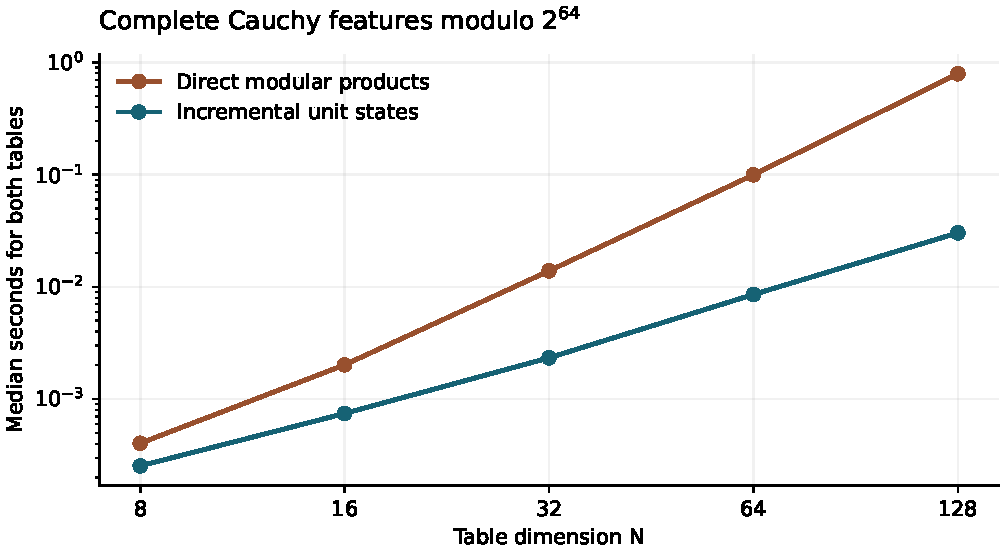
\includegraphics[width=.86\textwidth]{figures/benchmark.pdf}
\caption{Measured time for complete two-table construction with identical
64-bit output. The direct modular baseline isolates prefix reuse; these
are local kernel measurements, not SAT timings.}
\end{figure}

At $N=128$, the median drops from approximately $\matchedSlowSeconds$ seconds to
$\matchedFastSeconds$ seconds, a measured $\matchedSpeedup$-fold reduction. The trend is consistent
with the separately proved cubic-to-quadratic work reduction. Timings on
one shared machine do not establish universal speedup ratios.

The historical exact-rational implementation was also measured, including
conversion of its output to the same modular ring. At $N=32$, its median
is $\historicalSlowSeconds$ seconds against $\historicalFastSeconds$ seconds for the new method, a
$\historicalSpeedup$-fold ratio. That larger ratio includes both the arithmetic
representation change and prefix reuse; it should not be attributed
solely to the recurrence. Both benchmark series are retained.

\section{Integration, limitations, and further research}
\label{sec:future}

\subsection{A reviewable integration path}

The archive is a self-contained research packet. It supplies this PDF and
its complete LaTeX sources; the modular kernel; a matched direct-product
baseline; the unmodified historical Cauchy prototype and its repository
license; independent checks; exact schedule certificates; all measured
samples; and source pins and hashes. It makes no changes to the remote
repository. It can be filed under the existing research directory or
submitted through the user's usual incoming process.

For kernel integration, preserve the public meaning of the two feature
tables and compare residues at the caller's precision. Keep immutable
integer input lifts and valuation/unit states. The current module's ring
is quadratic; a production contractor must connect the same recurrence
to its actual unramified coefficient-ring interface. A large-field
implementation must preserve normalization before reduction, rather than
simply casting the quadratic prototype to another modulus.

For the polynomial-space bound, use the stated multistage arities and
retained-level fractions with the additive gap. For the optional cached
bound, use the separate eight-group schedule and account for its
subexponential storage. These are distinct resource choices. A finite
implementation should check every padding and precision inequality and
use the exact direct algorithm whenever the required finite inequalities
fail.

\subsection{What this iteration leaves open}

The report establishes an improved explicit contraction certificate and a
faster exact local kernel. It does not establish a better unrestricted
logarithmic order, a new end-to-end SAT implementation, a smaller numerical
coefficient per SAT variable, or an independent formal proof of the source
architecture. The optional cached construction spends additional space.
All of these distinctions matter to a fair comparison with the fifteen
packets.

The missing-interface proposals cannot be converted to theorems merely
by giving mode assignments shorter names. One must preserve group-local
structure, bound resulting tensor degrees, implement the sum, and pay for
all entry-oracle and bit operations. Similarly, exact Smith valuations
are a local constraint on changes of basis for a full padded block, not
a lower bound on SAT algorithms.

\subsection{Specific further questions}

\begin{enumerate}
\item \textbf{Optimize the entire feasible schedule.} The multistage
schedule is an explicit improvement, not a global optimizer. A rigorous
interval or rational branch-and-bound search over arities and cumulative
packet exponents could certify a better infimum or a useful restricted
optimality statement. Finite thresholds should be included in the objective.
\item \textbf{Exploit actual sparse ports.} Full-block Smith profiles are
sharp for the full padded orientation. Real packets may contain far fewer
ports. A decomposition using those sparse subsets might reduce mode counts
without violating source/target locality or making the oracle expensive.
\item \textbf{Avoid dense tables when few modes survive.} The new dense
algorithm is quadratic. A valuation-aware sparse API could output only
requested features or modes below the current precision budget, provided
it never discards a unit state that later reappears after a negative-valuation
update.
\item \textbf{Optimize the time-space tradeoff.} Eight groups and a
$3,3,2$ block split give a clean proof. Different splits, depth-dependent
caching, or bounded-memory recomputation could improve either resource
without invoking the unproved global summation oracle.
\item \textbf{Close a genuine order-changing interface.} Uniform
linear-wire compression, degree-preserving recursive factorization, or a
fully costed structured summation method remains the route to a stronger
logarithmic denominator. Any claimed solution should include its exact
representation and oracle costs.
\item \textbf{Formalize the new boundary.} The most contained next formal
lemmas are the unit-state recurrence, the missing-bit difference-set lemma,
and the compatibility of full-block modes with asymmetric child degrees.
They would reduce the trusted gap before attempting a formalized new
constant or a complete practical contractor.
\end{enumerate}

\section*{Reproduction guide}
\addcontentsline{toc}{section}{Reproduction guide}

From the extracted archive, run \path{python3 code/run_all.py}.
This uses only Python's standard library and writes fresh results into
\texttt{reproduced/}. It runs the modular and historical checks and all three
resource-certificate checkers. To repeat the timings, run
\path{python3 code/benchmark.py --historical vendor/joint_cauchy.py}.
The benchmark prints JSON; redirect it to a new file to preserve the
recorded samples. Run \texttt{make pdf} to rebuild the report from the
bundled LaTeX and figure. Regenerating the scientific figure additionally
requires Matplotlib; it is not required to run the verification or build
from the included vector PDF. No network access is needed for these steps.

\begin{thebibliography}{20}
\bibitem{proveit} Vladimir Reshetnikov et al. \emph{ProveIt: Sub-exponential
3-SAT}, pinned project index.\newline
\url{https://github.com/VladimirReshetnikov/ProveIt/blob/474ddba696a5d385c091c23fb2995f69edd13e00/Computability/SubexponentialSAT/README.md}.
\bibitem{incoming} ProveIt. \emph{New research reports}, commit introducing
seven additional ETH archives.\newline
\url{https://github.com/VladimirReshetnikov/ProveIt/commit/3e57705cf14ee9ac99c0ac35cfff751dcf70b396}.
\bibitem{openai} OpenAI. \emph{The Exponential Time Hypothesis is False},
October 25, 2026, pinned manuscript directory.\newline
\url{https://github.com/openai/math/tree/7ef5c0cc5ca4b0e072b7a050fca09ab24bc6fa3a/preprints/The-Exponential-Time-Hypothesis-is-False-October-25-2026}.
\bibitem{contraction} OpenAI. \emph{Quantitative contraction}, Appendix D
source, \texttt{build/quantitative-contraction.tex}, in \cite{openai}.
\bibitem{leanscope} OpenAI. \emph{Lean formalization scope},
\texttt{lean/docs/378.md}.\newline
\url{https://github.com/openai/math/blob/7ef5c0cc5ca4b0e072b7a050fca09ab24bc6fa3a/lean/docs/378.md}.
\bibitem{placed} ProveIt. Seven placed analysis packets, exact paths and
Git blob identifiers in this archive's \path{source_manifest.json};
\texttt{Computability/SubexponentialSAT/Research} at \cite{proveit}.
\bibitem{asymmetric} \emph{Asymmetric packet balancing for subexponential
SAT}, October 26, 2026. Incoming archive
\path{eth_asymmetric_packet_balancing_2026-10-26.zip} at \cite{incoming}.
\bibitem{joint} \emph{Full Crossing-Block Cauchy Modes}, October 26, 2026.
Incoming archive \path{eth_joint_cauchy_2026-10-26.zip} at \cite{incoming}.
\bibitem{roundtwo} \emph{Round-two refinement}, October 26--27, 2026.
Incoming archive \path{3sat_round2_refinement_20261027.zip} at \cite{incoming}.
\bibitem{matching} \emph{Matching Packing and Thin Gaps},
\path{eth_matching_refinement/report.tex}; arrival
\texttt{d098ba436b33df19365a44dd178694ff52845d19}, placed by
\texttt{6d3adc45061535ebe6fa7cd3d9b37dff7dcfc22a}.\newline
\url{https://github.com/VladimirReshetnikov/ProveIt/tree/474ddba696a5d385c091c23fb2995f69edd13e00/Computability/SubexponentialSAT/Research/eth_matching_refinement}.
\bibitem{otherincoming} The packet-refinement, balanced-packing,
high-moment and recursive-refinement packets in \cite{incoming}.
Full archive names, content hashes and report paths are in the source manifest.
\end{thebibliography}
\end{document}
